\documentclass{standalone}

\usepackage{setspace}
\usepackage{times}
\usepackage{amsmath}
\usepackage{amssymb}
\usepackage{xparse}
\usepackage{ifthen}

\usepackage[dvipsnames]{xcolor}
\usepackage{tikz}
\usetikzlibrary{arrows,calc,patterns,patterns.meta}
\usetikzlibrary{hobby,backgrounds}
\pgfdeclarelayer{background}
\pgfdeclarelayer{foreground}
\pgfsetlayers{background,main,foreground}

\usepackage{pgfplots}
\pgfplotsset{compat=1.15}

\renewcommand{\seriesdefault}{\bfdefault}
\renewcommand{\familydefault}{\sfdefault}

\definecolor{ocean}{HTML}{005EB8}

\begin{document}
    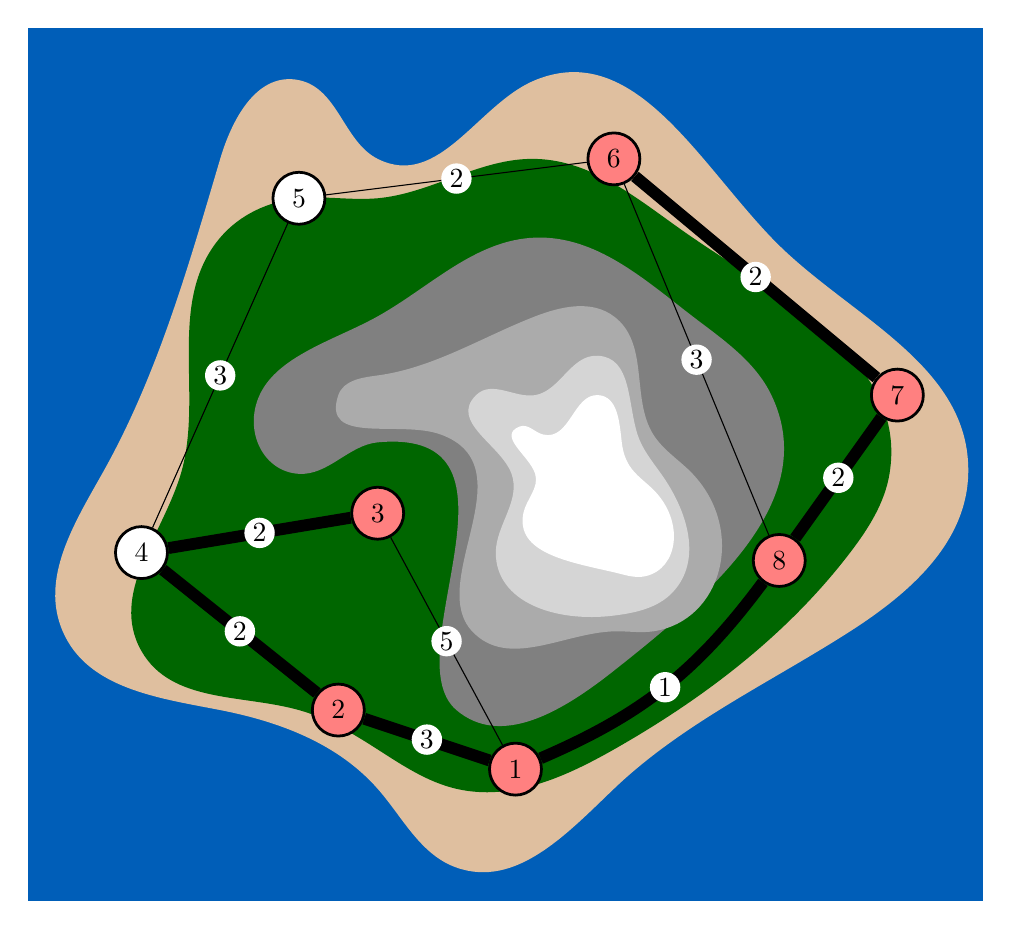
\begin{tikzpicture}[
		node/.style={circle,fill=white,draw,inner sep=0pt,line width=1pt, minimum size = 0.66cm},
		label/.style={circle,fill=white,inner sep=1pt},
		terminal/.style={fill=red!50!white},
		sol/.style={line width=1.5mm},
		background rectangle/.style={fill=ocean}, show background rectangle,
		]
		\draw[fill=brown!50!white,draw=none] (1,-1) to[closed, curve through = { (-1,-2) (-2,-1) (-4,0) (-6,1) (-5.5,3) (-4,7) (-3,8) (-2,7) (0,8) (3,6) (5.5,3) }] (4,1);
		\draw[fill=green!40!black,draw=none] (1,-0.5) to[closed, curve through = { (-1,-1) (-2,-0.5) (-3,0) (-5,0.75) (-4.5,3) (-4,6) (-3,6.5) (-2,6.5) (0,7) (2,6) (4.5,3) }] (4,2);
		\draw[fill=gray,draw=none] (1,0.5) to[closed, curve through = { (-1,0) (-2,3.4) (-3,3) (-3.5,4) (-3,4.5) (-2,5) (0,6) (2,5) }] (3,4);
		\draw[fill=gray!66!white,draw=none] (1,1) to[closed, curve through = { (-0.8,1) (-1.2,3.5) (-2.5,4) (-2,4.25) (0,5) (1,5) (1.5,3.5) (2,3) }] (1.5,1);
		\draw[fill=gray!33!white,draw=none] (1,1.2) to[closed, curve through = { (-0.5,2) (-0.3,3) (-0.75,4) (0,4) (0.8,4.5) (1.3,3.5) (1.6,3) }] (1.75,1.5);
		\draw[fill=white,draw=none] (1,1.75) to[closed, curve through = { (-0.15,2.5) (0,3) (-0.2,3.6) (0.1,3.5) (0.8,4) (1.1,3.4) (1.2,3.1) (1.5,2.8) }] (1.4,1.7);

		\node[node,terminal](n1) at (-0.25,-0.75) {$1$};
		\node[node,terminal](n2) at (-2.5,0) {$2$};
		\node[node,terminal](n3) at (-2,2.5) {$3$};
		\node[node         ](n4) at (-5,2) {$4$};
		\node[node         ](n5) at (-3,6.5) {$5$};
		\node[node,terminal](n6) at (1,7) {$6$};
		\node[node,terminal](n7) at (4.6,4) {$7$};
		\node[node,terminal](n8) at (3.1,1.9) {$8$};

		\draw[sol] (n1) --node[label,midway]{$3$} (n2);
		\draw      (n1) --node[label,midway]{$5$} (n3);
		\draw[sol] (n1) to[bend right=15] node[label,midway]{$1$} (n8);
		\draw[sol] (n2) --node[label,midway]{$2$} (n4);
		\draw[sol] (n3) --node[label,midway]{$2$} (n4);
		\draw      (n4) --node[label,midway]{$3$} (n5);
		\draw      (n5) --node[label,midway]{$2$} (n6);
		\draw[sol] (n6) --node[label,midway]{$2$} (n7);
		\draw      (n6) --node[label,midway]{$3$} (n8);
		\draw[sol] (n7) --node[label,midway]{$2$} (n8);

		% \fill[fill=gray!70!white] (1,2) -- (3,2) -- (3,4) -- (5,4) -- (5,1) -- (7,1) -- (7,5) -- (1,5) -- cycle;
		% \draw[draw=black,line width=0.1cm] (7,5) -- (1,5) -- (1,2) -- (5,2) -- (5,1) -- (7,1) -- cycle;
    \end{tikzpicture}
\end{document} 
